\documentclass[xcolor=svgnames,slideopt,A4,handout]{beamer}
\usepackage[english]{babel}
\usepackage[T1]{fontenc}
\usepackage[utf8]{inputenc}
\usepackage{microtype}
\usetheme{default}

\useoutertheme{infolines}
\usepackage{eso-pic}
\usepackage{monster2e}
\usepackage{tikz}
\usepackage{layout}
\usepackage{xcolor}
\usepackage{amsmath,amssymb}
\usepackage{fancybox}
\usepackage{graphicx}
% \usepackage{titling}
\usepackage[absolute,showboxes,overlay]{textpos}
\TPshowboxesfalse
\textblockorigin{0mm}{0mm}
\usepackage{appendixnumberbeamer}

\definecolor{rouge2}{RGB}{230,68,57}  % red S



\setbeamertemplate{navigation symbols}{}

\renewcommand{\sfdefault}{lmss}
\sffamily

\setbeamersize{text margin left=1cm,text margin right=1cm}

\setlength{\parindent}{0pt}
\setlength{\parskip}{6pt plus 2pt minus 1pt}
\setlength{\emergencystretch}{3em}  % prevent overfull lines
\setcounter{secnumdepth}{0}
\usepackage[citestyle=authoryear-comp,bibstyle=ieee,isbn=false,maxnames=1,minnames=1,sorting=nyt,backend=biber,defernumbers=true]{biblatex}

\AtEveryBibitem{
   \clearfield{arxivId}
   % \clearfield{booktitle}
   \clearfield{doi}
   \clearfield{eprint}
   \clearfield{eventdate}
   \clearfield{isbn}
   \clearfield{issn}
   % \clearfield{journaltitle}
   \clearfield{month}
   % \clearfield{number}
   \clearfield{pages}
   \clearfield{series}
   \clearfield{url}
   \clearfield{urldate}
   \clearfield{venue}
   % \clearfield{volume}
   \clearlist{location} % alias to field 'address'
   \clearlist{publisher}
   \clearname{editor}
}
\addbibresource{../../../biblio/magnet.bib}

\title{Correlation Clustering}
\author{Géraud Le Falher --- MAGNET}
\date{January 22, 2015}
\renewcommand{\theauthor}{Géraud Le Falher}
\newcommand{\shorttitle}{Clustering in signed graphs}

\begin{document}


%%%%%%%%%%%%%%%%%%%%%PREMIERE PAGE FOND INRIA

\setbeamertemplate{background canvas}{\includegraphics[width=\paperwidth,height=\paperheight]{premiere-sc-en}} 

\setbeamertemplate{footline}{ \hspace{5em} \textcolor{white} {\theauthor{} \hfill\today}\hspace{2em}\null \vspace*{3pt}}


\begin{frame}

\begin{textblock*}{7cm}(13mm,50mm)
	{\textcolor{white} {
			{\huge Clustering and sign prediction in signed graphs}%\\[2mm]
			% { \huge 2 LIGNES MAXIMUM}\\[3mm]
			% {\Large Sous-titre facultatif}%
		}
	}
	\end{textblock*}

\vspace*{-4pt}
\end{frame}


% \setbeamertemplate{background canvas}{\includegraphics[width=\paperwidth,height=\paperheight]{fondrouge}} 
% \setbeamertemplate{footline}{
% \hspace{2cm} 
% \raisebox{2.5ex}
%   {\textcolor{white}{\theauthor{} -- \shorttitle{}}}\hfill 
%   \raisebox{2.5ex}
%   {\textcolor{white}{\insertframenumber~/~\inserttotalframenumber \hspace{1em}}}}
%
% \setbeamercolor{frametitle}{fg=White}
% \begin{frame}{Introduction}
%
% \begin{textblock*}{10cm}(20mm,20mm)
% \textcolor{white}
% 	{Your text with scientific results or what ever... Your text with
% scientific results or what ever... Your text with scientific results or
% what ever... Your text with scientific results or what ever... Your
% text with scientific results or what ever... Your text with scientific
% results or what ever... Your text with scientific results or what
% ever... Your text with scientific results or what ever... Your text
% with scientific results or what ever...}
%
% \textcolor{white}{Your text with scientific results or what ever... Your text with
% scientific results or what ever... Your text with scientific results or
% what ever... Your text with scientific results or what ever... Your
% text with scientific results or what ever... Your text with scientific
% results or what ever... Your text with scientific results or what
% ever.}
%
% \end{textblock*}
%
%
% \end{frame}
%%%%%%%%%%%%%%%%%%%%%%%%%%%



\setbeamertemplate{background canvas}{\includegraphics[width=\paperwidth,height=\paperheight]{basrouge}} 
\setbeamertemplate{footline}{
\hspace{2cm} 
\raisebox{2.5ex}
  {\textcolor{white}{\theauthor{} -- \shorttitle{}}}\hfill 
  \raisebox{2.5ex}
  {\textcolor{white}{\insertframenumber~/~\inserttotalframenumber \hspace{1em}}}}


\begin{frame}{Outline}
\tableofcontents
\end{frame}




%%%%%%%%%%%%%%%%%%%%%%%%%%%

% \setbeamertemplate{background canvas}{\includegraphics[width=\paperwidth,height=\paperheight]{fondrouge+tab}} 
%
% \setbeamertemplate{footline}{
% \hspace{2cm} 
% \raisebox{2.5ex}
%   {{\theauthor{} -- \shorttitle{}}}\hfill 
%   \raisebox{2.5ex}
%   {{\today - \insertframenumber \hspace{5mm} \null }}}
%
% \begin{frame}
%
%
%
% \begin{textblock*}{7cm}(13mm,40mm)
% {\textcolor{white} {
% {\monster 1}\\[2mm]
%    { \huge PREMIER CHAPITRE}\\[3mm]
%    	{\Large Sous-titre facultatif}}
% 	}
% 	\end{textblock*}
%
% \vspace*{-4pt}
% \end{frame}

%%%%%%%%%%%%%%%%%%%%%


\setbeamertemplate{background canvas}{\includegraphics[width=\paperwidth,height=\paperheight]{basrouge}} 

% \setbeamertemplate{footline}{
% \hspace{2cm} 
% \raisebox{2.5ex}
%   {\textcolor{white}{\theauthor{} -- \shorttitle{}}}\hfill 
%   \raisebox{2.5ex}
%   {\textcolor{white}{\today - \insertframenumber \hspace{5mm} \null }}}


\begin{frame}{Problem}
\section{Problem}

\begin{block}{input}

\begin{itemize}
\itemsep1pt\parskip0pt\parsep0pt
\item
  \(n\) objects
\item
  partial pairwise binary information
\end{itemize}

\end{block}

\begin{block}{output}

clustering

\end{block}

\begin{block}{measure of quality}

\begin{itemize}
\itemsep1pt\parskip0pt\parsep0pt
\item
  disagreement edges
\item
  minimize their number
\end{itemize}

\end{block}

\end{frame}

\begin{frame}
		\includegraphics[height=0.8\textheight]{signed_network.pdf}
\end{frame}
\begin{frame}{Comparison with other clustering problems}

\begin{itemize}
\itemsep1pt\parskip0pt\parsep0pt
\item
  the number of clusters is part of the solution. If $k$ is fixed, PTAS in
  $n^{O(\frac{9^k}{\epsilon^2})}\log(n)$ \autocite{Giotis2006}
\item
  it does not require a distance between objects
\end{itemize}

\end{frame}

\begin{frame}{Applications}
\section{Applications}

	2 keys applications in social graphs:
	\begin{itemize}
		\itemsep1pt\parskip0pt\parsep0pt
		\item find antagonistic groups in signed graphs or in users/items
			bipartite graph \autocite{Bipartite12}
		\item predict sign of unknown link \autocite{Leskovec2010} (why?)
	\end{itemize}
\end{frame}

\begin{frame}
	\begin{figure}[h]
		\centering
		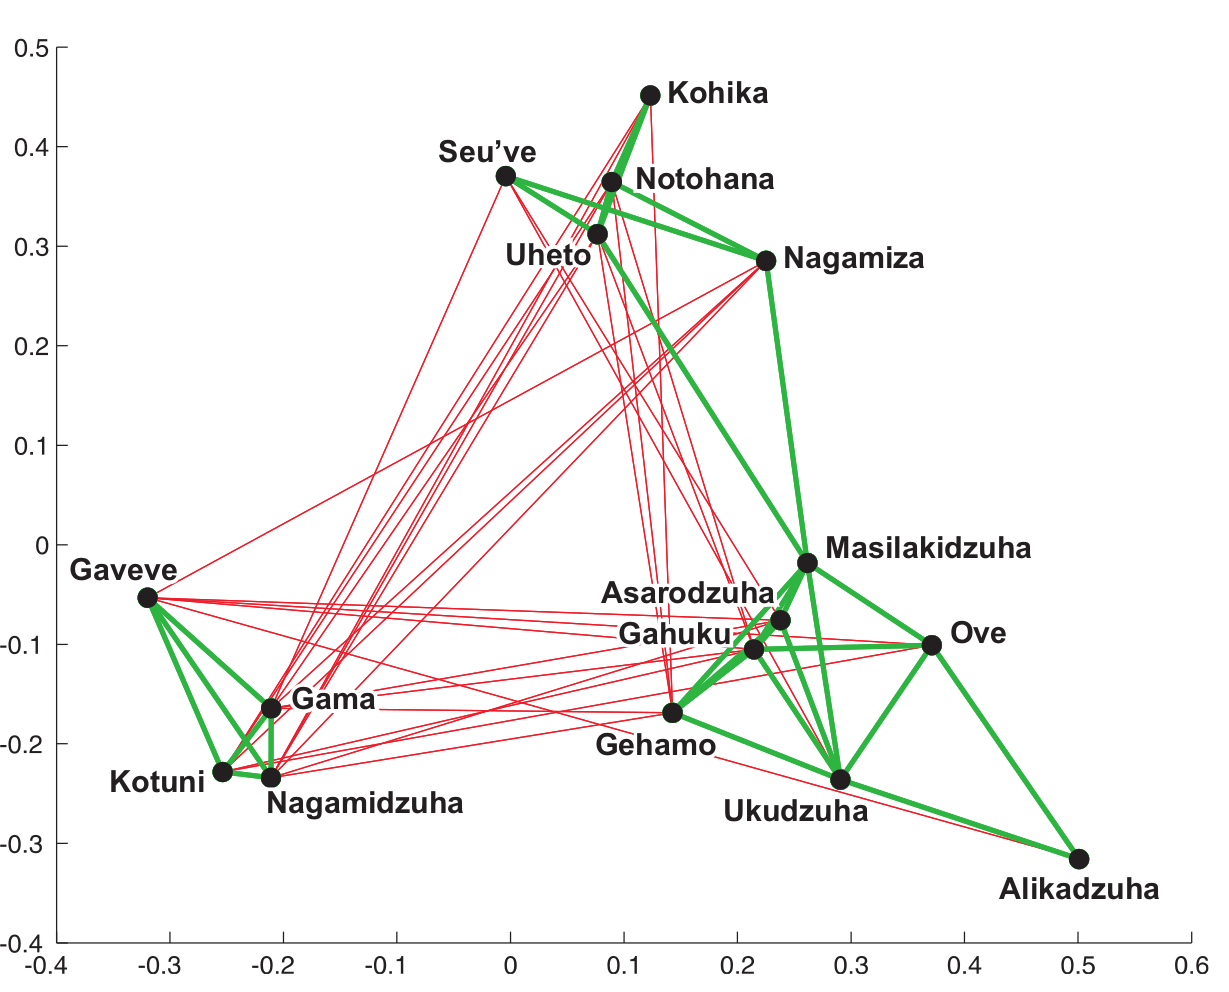
\includegraphics[width=0.8\linewidth]{tribes.png}
		\caption{Tribes \autocite{Luca10}}
	\end{figure}
\end{frame}

\begin{frame}
	\begin{figure}[h]
		\centering
		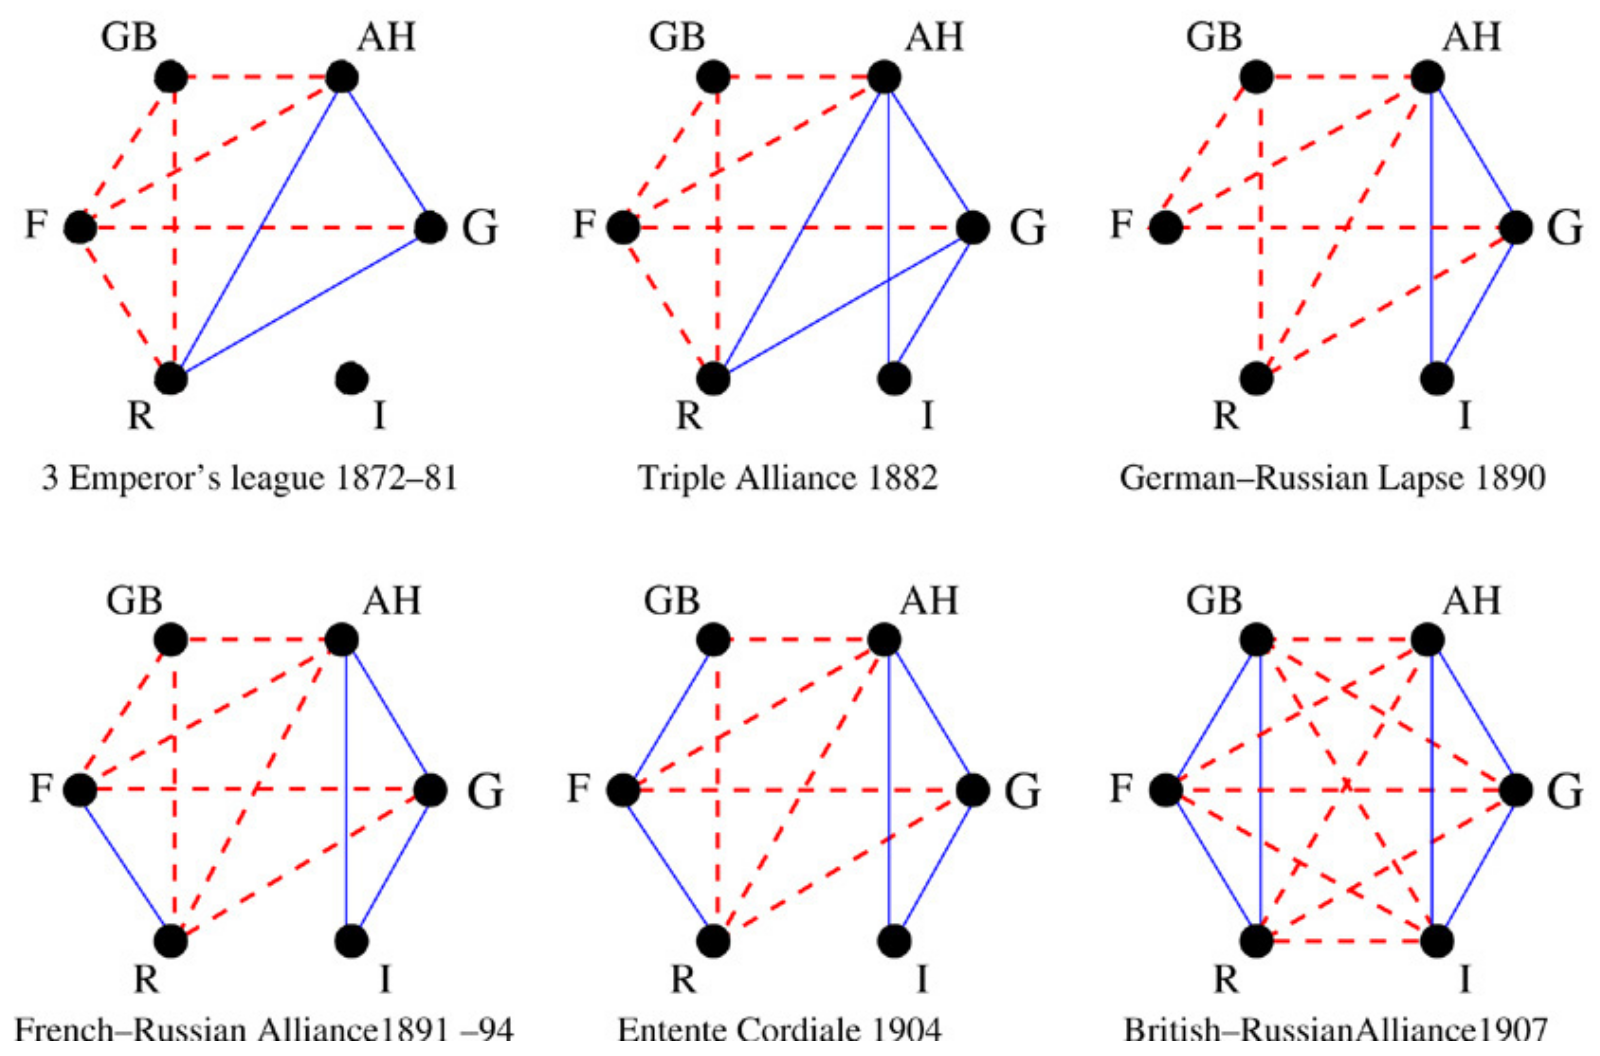
\includegraphics[width=0.8\linewidth]{europe.png}
		\caption{Military alliances before WW1 \autocite{Antal2006a}}
	\end{figure}
\end{frame}

\begin{frame}
	\begin{figure}[h]
		\centering
		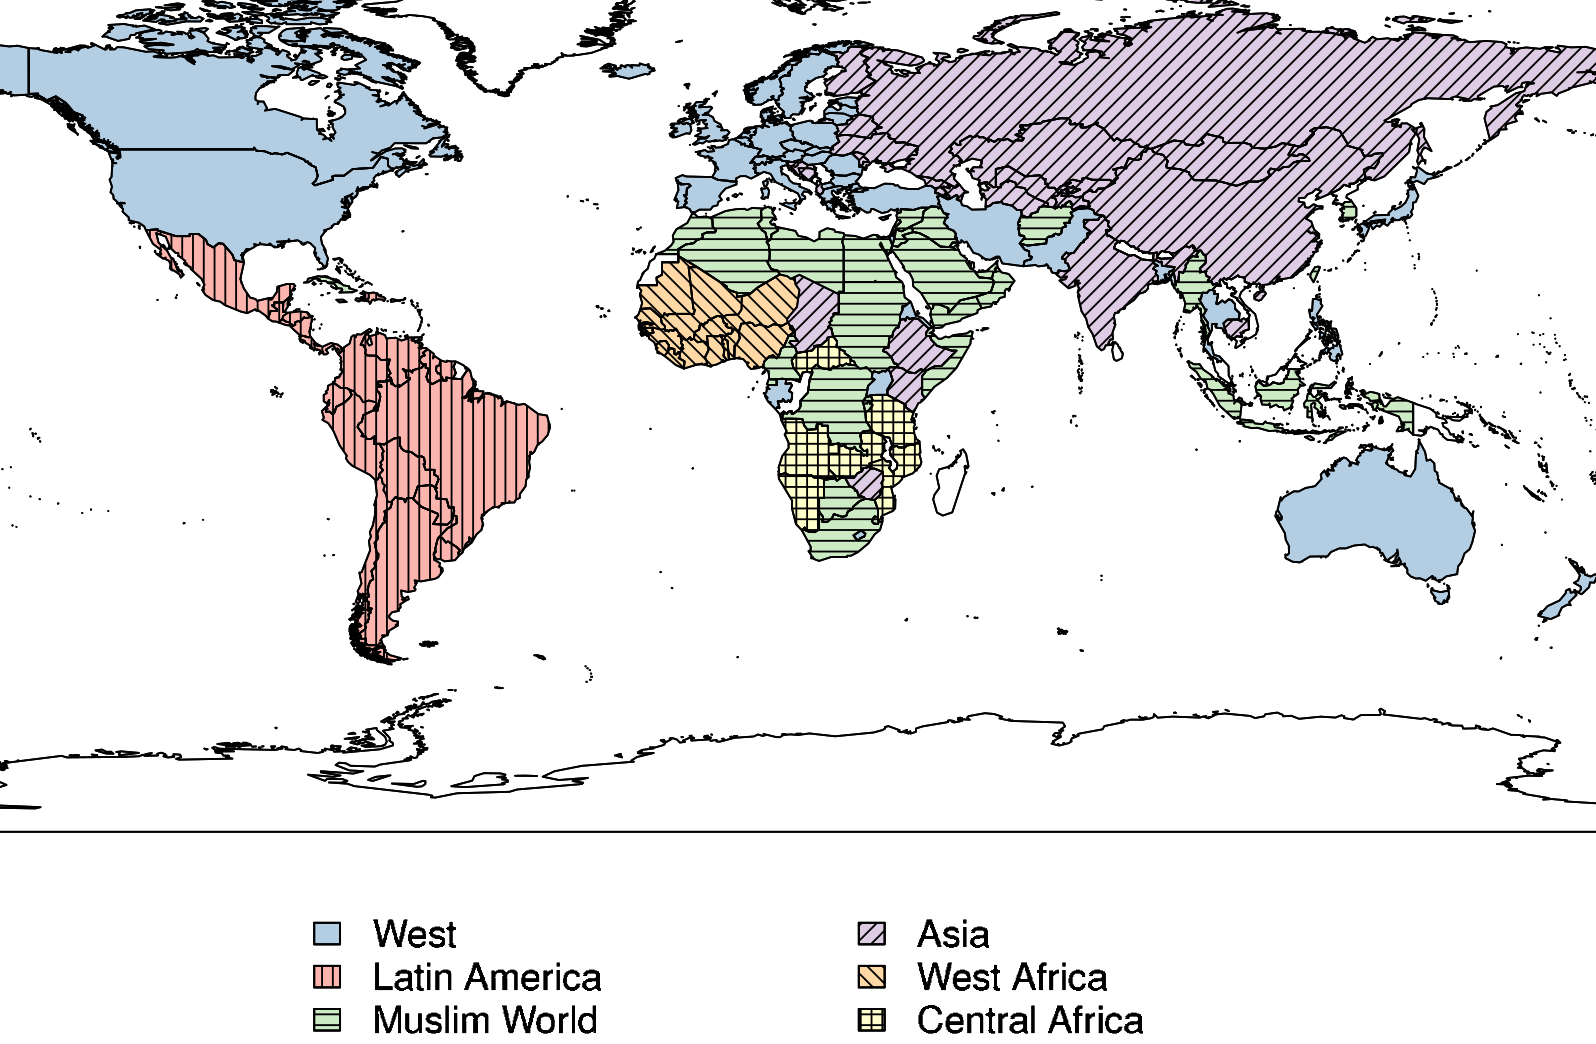
\includegraphics[width=0.8\linewidth]{world.png}
		\caption{Correlates of war between 1993 and 2001 \autocite{Traag2009}}
	\end{figure}
\end{frame}

\begin{frame}{Applications}
		In other domains:
	\begin{itemize}
		\itemsep1pt\parskip0pt\parsep0pt
		\item
			Biology: Functional analysis of signed co-expression networks of genes
			\autocite{Mason2009}
		\item
			NLP: coreference \autocite{graphicalCoreference04}
		\item
			Web: Entity resolution \autocite{DeDup09}
	\end{itemize}
\end{frame}
\begin{frame}{State of the art}
	\section{State of the art}
	
	\begin{block}{Complete graph}
		Easiest because information on all pairs. Yet it is NP-complete by
		reduction from multicut \autocite{Demaine2006}.

		There is a quadratic combinatorial randomized approximation with expected
		cost at most 3 times the optimal \autocite{Ailon2008}.

		while not all nodes are clustered
		\begin{itemize}
			\itemsep1pt\parskip0pt\parsep0pt
			\item
				choose a node at random
			\item
				put it in a new cluster along with its positive neighborhood and remove
				them from the original graph
		\end{itemize}

	\end{block}
\end{frame}

\begin{frame}{State of the art}
	\begin{block}{General graph}
		More ambiguous, thus more difficult: There is a polynomial
		approximation (with ratio $O(\log n)$) that solve the following linear
		program \autocite{Demaine2006}, but for any constant $c$, getting a
		$O(c)$ approximation is NP-Hard.

		\begin{align*}
			\min \sum_{(i,\, j)\in E^+} (1-x_{ij}) w_{ij} +
			\sum_{(i,\, j)\in E^-} x_{ij} w_{ij} \\
			x_{ij} =   \begin{cases}
				1 & \text{if $i$ and $j$ are in the same cluster} \\
				0       & \text{otherwise}
			\end{cases} \\
			x_{ij} \in [0,\,1]
		\end{align*}
	\end{block}

\end{frame}
\begin{frame}{State of the art}
	\begin{block}{General graph}
Other approaches include spectral clustering \autocite{Luca10} and communities
detection \autocite{Yang2007} tailored to signed graphs.
	\end{block}
\end{frame}

\begin{frame}{Our solution for general graph}
	\section{Our method (so far)}
	first complete the graph in a combinatorial fashion, run Ailon algorithm
	and keep the clustering induced on the original graph.

	Our hope is to get $O(\log n)$ approximation in worst case and better for
	\enquote{realistic average-case} \autocite{Makarychev2014} with a
	reasonably polynomial complexity.

	mildly satisfying experimental results
\end{frame}
\appendix
\begin{frame}[t,allowframebreaks]
	\frametitle{References}
	\printbibliography
\end{frame}

%%%%%%%%%%%%%%%%%%%%%%%%%%%


\setbeamertemplate{background canvas}{\includegraphics[width=\paperwidth,height=\paperheight]{derniere-sc-en}} 
\setbeamertemplate{footline}{}


\begin{frame}

\begin{center} 
\textcolor{white} {\huge Thank you for your attention}
\end{center}
\begin{center} 
\textcolor{white} {\Large Questions?}
\end{center} 

% \begin{textblock*}{7cm}(60mm,76mm)
% {\textcolor{white} {
% {LIEU}\\[1mm]
%    {LOCALISATION}\\[2mm]
%    	{www.nomdedomaine.com}}
% 	}
% 	\end{textblock*}
%
%
% \vspace*{-4pt}
\end{frame}
\end{document}

